\section{Worked Example: The Impact of AI Coding Tools in Open-Source Projects}
\label{sec:worked-example}

The preceding sections introduced the causal inference toolkit at a conceptual level---defining estimands, encoding assumptions in DAGs, and outlining design-based identification strategies.
We now put these ideas to work on a concrete empirical problem.
Using a dataset of popular open-source GitHub repositories, we ask: \emph{Does the systematic adoption of AI coding tools increase a project's development velocity?}\footnote{The choice of this worked example is partially motivated by the authors' own prior work~\cite{DBLP:conf/msr/HeMAKV26}, but we deliberately tailored the worked example to be more up-to-date and more illustrative of our thought process that arrived at a more credible causal inference design presented in the original paper.}
We introduced this question in Section~\ref{sec:primer-causality} and used it throughout Section~\ref{sec:primer} to motivate each pillar of the toolkit; here, we get our hands dirty with real data.
Rather than presenting a single analysis and defending its conclusions, we walk through a \emph{progression} of methods---each motivated by the specific inadequacy of the previous one---to illustrate how the toolkit guides a researcher from a na\"ive comparison to a credible causal design.
The goal is not to produce a definitive causal estimate of AI coding tools' impact---no single observational study can---but to demonstrate the full arc of a credible causal inquiry: how a researcher should reason about design choices, what they should worry about, and how they should communicate the strength of their evidence.

\subsection{Study Setting}
\label{sec:study-setting}

\paragraph{Research Question and Target Trial.}
In Section~\ref{sec:primer-causality}, we sketched the target trial for this question: randomly assign half of a set of comparable software projects to adopt AI coding tools and compare monthly commits after a fixed period.
We now operationalize each component of this target trial using observational data from GitHub.
The population is popular open-source repositories.
The treatment is systematic AI coding tool adoption, as signaled by AI configuration files committed to the repository.
The outcome is the monthly commit count on the default branch, used as a proxy for development velocity.
Articulating the target trial immediately surfaces the threats we must address: We cannot randomly assign tool adoption (selection bias); the ``treatment'' bundles multiple distinct interventions (the compound treatment concern from Section~\ref{sec:primer-stance}); and commit counts are a noisy proxy for the latent construct of development velocity (the measurement concern from Section~\ref{sec:primer-stance}).
The remainder of this subsection describes how we construct the dataset and discusses the implications of each operationalization choice.

\paragraph{Corpus Construction.}
We sample repositories from GitHub, the largest host of open-source software, using a stratified design across 10 widely used programming languages: Python, JavaScript, TypeScript, Java, C++, C, Go, Rust, Ruby, and Swift.
For each language, we query the GitHub Search API for the top 100 non-fork, non-archived repositories ranked by star count, yielding a corpus of 1,000 repositories.
For each repository, we collect cross-sectional metadata available through the GitHub REST and GraphQL APIs: star count, fork count, open issue count, repository size, creation date, owner type (user vs.\ organization), total commit count, total pull request count, total issue count, total release count, and whether the repository has continuous integration workflows and discussion forums enabled.

To support the longitudinal analysis in Section~\ref{sec:longitudinal}, we construct a monthly panel spanning 27 months (January 2024 through March 2026) for each repository.
We clone each repository and mine its git history to extract two outcome measures per repository-month: the number of commits and the number of unique active contributors (distinct author email addresses).
To identify treatment timing, we scan the git history for the earliest commit that added an AI configuration file, using the author date of that commit as the treatment date; this allows us to determine precisely when each repository transitioned from untreated to treated, which is essential for the before-and-after and difference-in-differences designs.
We enrich the panel with time-varying covariates from the GHArchive public dataset via BigQuery, aggregating monthly counts of new stars, issues opened, forks, pull requests merged, and releases for each repository.
These time-varying covariates serve dual roles in the analysis: as potential confounders in the longitudinal models (Section~\ref{sec:did}) and as concrete examples of the temporal collapse problem when measured cross-sectionally (Section~\ref{sec:temporal-collapse}).
All data collection scripts are available in the replication package (Section~\ref{sec:data-availability}).

\paragraph{Treatment: Systematic AI Coding Tool Adoption.}
We operationalize AI coding tool adoption by scanning each repository's file tree for configuration files associated with AI coding assistants.
These files---such as \Code{AGENTS.md}, \Code{CLAUDE.md}  (Anthropic Claude), \Code{.cursorrules} and \Code{.cursor/rules/} (Cursor), and \Code{.github/copilot-instructions.md} (GitHub Copilot)---provide repository-specific instructions, coding conventions, and context to AI tools, signaling that the development team has made a deliberate decision to integrate AI coding assistants into their workflow.
The full list of file-path patterns used for classification is available in the replication package (Section~\ref{sec:data-availability}).
A repository is \emph{treated} if it contains any such AI configuration artifacts and \emph{untreated} otherwise.
%As a supplementary treatment signal, we also scan each repository's contributor list for known AI bot accounts (e.g., accounts associated with Claude, Devin, CodeRabbit, or Copilot), which provide additional evidence of AI tool integration beyond configuration files.

\paragraph{Outcome: Development Velocity.}
We measure development velocity using monthly commit counts, extracted from the git history of each repository across the 27-month panel window.
Commit count is a standard---albeit imperfect---proxy for development activity in mining software repositories research: It is readily available, consistently defined across repositories, and captures a meaningful dimension of development effort.
However, commit counts conflate substantively different activities (feature development, bug fixes, documentation updates, automated commits) and can be inflated by CI-generated or bot-generated commits.
As Section~\ref{sec:primer-stance} emphasized, measurement and identification are orthogonal challenges: A perfectly identified design still produces misleading conclusions if the outcome proxy is invalid.
We proceed with monthly commits as the primary outcome while acknowledging this limitation; researchers applying these methods to their own settings should invest in validating and triangulating their outcome proxies.

\paragraph{What Does This Treatment Identify?}
The treatment variable deserves careful scrutiny, because it determines the estimand's substantive interpretation.
The presence of AI configuration files does not merely signal that individual developers use AI coding tools---such use is widespread and leaves no trace in the repository.
Rather, it signals that the team has invested effort in integrating AI tools at the project level: writing repository-specific instructions, establishing AI-related conventions, and in some cases deploying autonomous AI agents for triage, code review, or code generation.
This is precisely the \emph{compound treatment} concern raised in Section~\ref{sec:primer-stance}: What we estimate is the effect of the \emph{entire bundle}---the AI tools themselves, the workflow reorganization that accompanies structured adoption, and the team characteristics that lead to early adoption---not the isolated effect of AI tools alone.
A positive estimated effect does not mean that ``just using AI tools'' increases velocity; it means that the constellation of practices accompanying systematic AI integration is associated with---or, under stronger identification, causes---higher development velocity.

This framing is deliberate.
We do not attempt to measure the effect of ``using AI coding tools'' in general---an ill-defined treatment that would require knowing whether each individual developer uses one of the AI coding tools, which is unobservable from GitHub data and would introduce severe measurement error if we were to only collect partial traces of AI tool usage from one or two tools.
Instead, we define the treatment as \emph{systematic, project-level AI integration}, which is directly observable through committed configuration files and represents a substantively meaningful intervention: the decision to restructure a project's workflow around AI tools.
The contrast we estimate---systematic adoption versus no systematic adoption---is well-defined and practically relevant, because it is exactly the organizational decision that engineering leaders face.
This cleaner treatment definition does not eliminate measurement error entirely.
Repositories without configuration files may still have developers who use AI coding tools individually, contaminating the control group with unmeasured individual-level AI use.
This misclassification is asymmetric: Treated repositories are likely genuine systematic adopters, but some control repositories contain individual AI users.
The standard consequence is \emph{attenuation bias}---the estimated treatment effect is biased toward zero because the contrast between treated and control groups is blurred~\cite{hausman2001mismeasured}.
Attenuation bias means our estimates would be conservative and lower than the effect of systematic AI coding tool adoption compared to not using AI at all.

\paragraph{Population and External Validity.}
Our sampling strategy---selecting the most-starred repositories per language---produces a diverse corpus of highly visible, actively maintained open-source projects.
This population is deliberately unrepresentative of the ``average'' GitHub repository, most of which are small, single-developer, or dormant.
The trade-off is intentional.
Popular repositories offer sustained development activity, meaningful commit histories, and observable adoption signals---properties required for any analysis to be informative.
A random sample of all GitHub repositories would suffer from severe floor effects (most repos have near-zero monthly commits) and sparse treatment prevalence (AI configuration files are rare outside well-maintained projects), yielding a dataset with little statistical power and questionable practical relevance.
This is an instance of the tension between internal and external validity discussed in Section~\ref{sec:primer-stance}: We restrict the study population to improve data quality and the plausibility of the identification strategy, at the cost of generalizability.
The resulting estimates speak to the effect of systematic AI adoption among popular, actively maintained open-source projects---the segment where AI tools are being integrated most visibly and where the stakes of adoption decisions are highest.
Whether the same dynamics hold for smaller, less visible, or proprietary projects is an open question that lies outside the scope of this worked example but constitutes a natural direction for future research.

\subsection{Cross-Sectional Methods}
\label{sec:cross-sectional}

We begin with the approach commonly seen in mining software repositories studies, in which the researcher may: (1) start with a comparison of treated and control repositories using a cross-sectional snapshot, and then (2) run a regression with all available covariates, and interpret the surviving coefficient as suggestive evidence of an effect.
We then use the toolkit from Section~\ref{sec:primer} to diagnose the problems with this approach and show a DAG-justified regression with pre-treatment covariates and the use of two more sophisticated estimators (i.e., propensity score matching and inverse probability weighting).
Finally, we will use the same toolkit to demostrate the foundamental limitation of unobserved confounders to motivate the use of longitudinal data and design based identification.

\subsubsection{Na\"ive Group Comparison}
\label{sec:naive-comparison}

\begin{table}[t]
  \centering
  \begin{threeparttable}
  \caption{Descriptive comparison of treated (AI config present) and control (no AI config) repositories.
  SMD = standardized mean difference; $|\text{SMD}| > 0.1$ indicates meaningful imbalance and $|\text{SMD}| > 0.25$ indicates significant imbalance~\cite{austin2009balance}.
  Covariates are classified by temporal status: ``pre-treatment'' variables are determined at creation and cannot be affected by AI adoption under any timing; ``time-varying'' variables accumulate before and after adoption, making their cross-sectional values temporally ambiguous (Section~\ref{sec:temporal-collapse}).
  All count variables are log-transformed with $\log(1+x)$ to address skewness.}
  \label{tab:descriptive}
  \small
  \begin{tabular}{lrrrlrrr}
  \toprule
  \multicolumn{4}{c}{Pre-treatment\tnote{a}} & \multicolumn{4}{c}{Time-varying} \\
  \cmidrule(r){1-4} \cmidrule(l){5-8}
  Variable & Control Mean & Treated Mean & SMD & Variable & Control Mean & Treated Mean & SMD \\
  \midrule
  Repo age (yr) & 9.36 & 7.73 & $-$0.370 & \textbf{Avg monthly commits} & \textbf{71.38} & \textbf{412.38} & \textbf{0.309} \\
  Org.\ owner\tnote{b} & 0.65 & 0.81 & 0.366 & log(Stars) & 10.32 & 10.66 & 0.441 \\
  C & 0.12 & 0.04 & $-$0.294 & log(Forks) & 8.15 & 8.57 & 0.388 \\
  C++ & 0.11 & 0.07 & $-$0.115 & log(Size KB) & 10.47 & 11.88 & 0.754 \\
  Go & 0.09 & 0.14 & 0.148 & log(Total commits) & 7.89 & 9.06 & 0.743 \\
  Java & 0.11 & 0.06 & $-$0.201 & log(Total PRs) & 6.78 & 8.35 & 0.911 \\
  JavaScript & 0.11 & 0.07 & $-$0.115 & log(Total issues) & 6.92 & 7.85 & 0.461 \\
  Python & 0.10 & 0.11 & 0.023 & log(Releases) & 3.12 & 4.32 & 0.610 \\
  Ruby & 0.10 & 0.09 & $-$0.034 & log(Open issues) & 5.13 & 5.78 & 0.378 \\
  Rust & 0.09 & 0.13 & 0.130 & Has CI/CD & 0.80 & 0.96 & 0.540 \\
  Swift & 0.11 & 0.06 & $-$0.201 & Has wiki & 0.58 & 0.40 & $-$0.348 \\
  TypeScript & 0.06 & 0.23 & 0.499 & Has discussions & 0.53 & 0.64 & 0.223 \\
  \bottomrule
  \end{tabular}
  \begin{tablenotes}\footnotesize
  \item[a] We make a simplifying assumption that organization ownership and primary language is pre-treatment with the intuition that both should be very rare for mature and established repositories in our observed time window (2024 - 2026). Technically, both can change over time (repositories may transfer between owners, and the primary language label may shift as the codebase evolves).
  \item[b] Proportion of repositories owned by a GitHub organization rather than a personal account.
  \end{tablenotes}
  \end{threeparttable}
\end{table}

Following the approach outlined in Section~\ref{sec:primer-naive}, we start by comparing the treated (repositories with AI configuration files) and control (repositories without) groups on the outcome and all available covariates.
Table~\ref{tab:descriptive} presents this comparison, with covariates classified by their temporal status---a distinction we motivate below.
The raw gap is enormous: Treated repositories average 412 monthly commits versus 71 for controls---a nearly 6$\times$ difference (SMD $= 0.31$).
But the imbalance extends far beyond the outcome.
Every covariate exceeds the conventional $\pm 0.1$ SMD threshold for balance, with many far exceeding it.
Treated repositories are younger (7.7 vs.\ 9.4 years), larger in codebase size (SMD $= 0.75$), and more likely to be organization-owned (81\% vs.\ 65\%); they have more stars, forks, pull requests (SMD $= 0.91$), issues, and releases; and they are far more likely to have CI/CD pipelines (96\% vs.\ 80\%).
The programming language distribution also differs markedly: TypeScript and Go repositories are heavily represented among adopters, while C and Swift barely participate.
These are not random differences but rather reflect a coherent selection mechanism: Well-resourced, actively maintained, organization-backed projects are the ones that adopt AI tools.
A na\"ive analyst might interpret the 6$\times$ raw gap in monthly commits as evidence that AI tools boost productivity, but Section~\ref{sec:primer-naive} explained why such comparisons conflate any genuine effect with selection bias.

\paragraph{Kitchen-Sink Regression.}
\label{sec:kitchen-sink}

A typical SE researcher would now run a multivariate regression controlling for everything available---the ``kitchen-sink'' approach.
We regress $\log(\text{monthly commits})$ on the treatment indicator and all cross-sectional covariates: repository age, programming language, organization ownership, CI/CD presence, stars, forks, repository size, pull requests, issues, and releases.
The coefficient on AI adoption is $0.946$ ($\text{SE} = 0.116$, $p < 0.001$, $R^2 = 0.59$), surviving a battery of controls.
A researcher following standard empirical SE practice might stop here and conclude that \emph{AI adoption is associated with \textbf{157.5\%} (i.e., $e^{0.946} - 1$) higher development velocity, holding all observables constant}, with a disclaimer in the limitation section to note that correlation does not imply causation and the evidence presented is only suggestive.
In this tutorial, we are going to push one step further: \textbf{Under what assumptions can this 157.5\% estimate be interpreted as a causal effect? Are these assumptions plausible?}

\subsubsection{The Temporal DAG}
\label{sec:temporal-dag}

Recall in Section~\ref{sec:primer-po} that the formal identifying assumption for linear regressions to carry a causal interpretation is conditional ignorability according to the potential outcomes framework.
Also recall in Section~\ref{sec:primer-dags} that causal DAGs and the back-door criterion provides a principled rule for the researcher to argue whether the covariates have been appropriately selected to satisfy the conditional ignorability assumption.
We have already provided an example DAG in Figure~\ref{fig:ai-dag} for illustrative purposes but the sharp reader may have already noticed that the DAG is ambiguous without accounting the temporal nature of software repository data.
Here, we resolve this ambiguity and constructing a proper \emph{temporal DAG} that describes what might be a plauible causal theory (Figure~\ref{fig:temporal-dag}).

Consider Popularity as an example.
In the true data-generating process, Popularity accumulate over time, so the actual causal DAG has time-indexed nodes:
\begin{itemize}[leftmargin=15pt]
    \item $\text{Popularity}_{t-1}$ (\emph{before} AI adoption) is a \textbf{confounder}: Popular projects attract AI-savvy contributors ($\text{Popularity}_{t-1} \to \text{Adoption}_t$) \emph{and} have more active contributor bases ($\text{Popularity}_{t-1} \to \text{Dev. Velocity}_t$).
    \item $\text{Popularity}_{t+1}$ (\emph{after} AI adoption) is a \textbf{collider}: Both AI adoption and high commit activity may increase a project's visibility and help attract more attention ($\text{Adoption}_t \to \text{Popularity}_{t+1} \leftarrow \text{Dev. Velocity}_t$).
\end{itemize}
In this temporal DAG, the adjustment set is unambiguous: Condition on $\text{Popularity}_{t-1}$, never on $\text{Popularity}_{t+1}$.
The same logic applies to every time-varying characteristic: Issues, forks, PRs, releases, repository size, and contributor count are each confounders in their pre-treatment incarnation and colliders in their post-treatment incarnation.

Figure~\ref{fig:temporal-dag} presents the full temporal DAG for our setting.
We group the time-varying covariates into four high-level concepts---\emph{Popularity} (stars), \emph{Demand} (issues), \emph{Activity} (forks, PRs, commits, releases), and \emph{Team Size} (active contributors)---and split each into a pre-treatment node (confounder) and a post-treatment node (collider).
The structurally pre-treatment confounders---Domain (programming language), Organization (owner type), and Project Maturity (repo age)---remain as in Figure~\ref{fig:ai-dag}, along with Team Skill, which is entirely unobserved.
The causal paths run through two mediators: Code Generation and Workflow Automation.
Applying the back-door criterion (Section~\ref{sec:primer-dags}) to this temporal DAG yields an unambiguous adjustment set: All pre-treatment nodes (both structurally pre-treatment and time-varying-before-treatment) are confounders that must be conditioned on; all post-treatment nodes are colliders that must not be conditioned on; and the mediators must not be conditioned on because they lie on the causal path.

\begin{figure}[t]
\centering
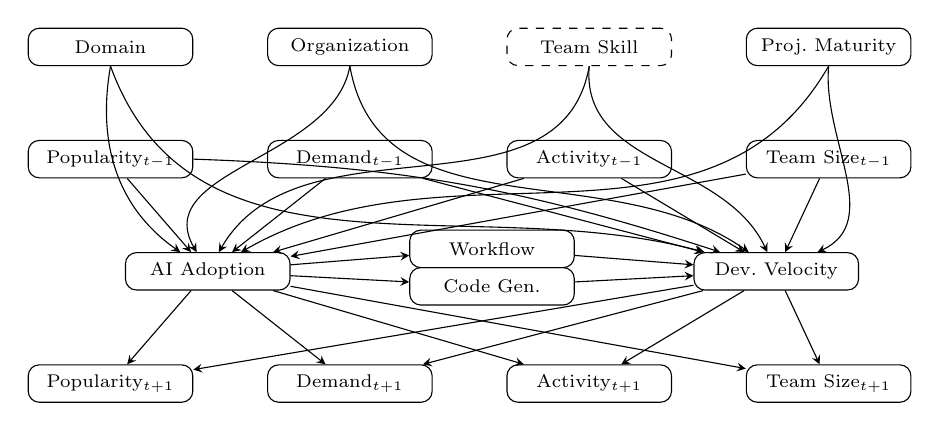
\begin{tikzpicture}[
    var/.style={draw, rounded corners, minimum width=2.2cm, minimum height=0.5cm, font=\scriptsize, align=center},
    unobs/.style={draw, rounded corners, dashed, minimum width=2.2cm, minimum height=0.5cm, font=\scriptsize, align=center},
    arr/.style={->, >=stealth, thin},
    scale=0.95, transform shape
]
\pgfdeclarelayer{bg}
\pgfsetlayers{bg,main}
% Structural pre-treatment confounders (top row)
\node[var] (domain) at (0, 3.5) {Domain};
\node[var] (org) at (3.2, 3.5) {Organization};
\node[unobs] (skill) at (6.4, 3.5) {Team Skill};
\node[var] (maturity) at (9.6, 3.5) {Proj.\ Maturity};

% Pre-treatment time-varying confounders (second row)
\node[var] (pop_pre) at (0, 2) {Popularity$_{t\text{-}1}$};
\node[var] (demand_pre) at (3.2, 2) {Demand$_{t\text{-}1}$};
\node[var] (activity_pre) at (6.4, 2) {Activity$_{t\text{-}1}$};
\node[var] (team_pre) at (9.6, 2) {Team Size$_{t\text{-}1}$};

% Main causal chain (middle)
\node[var] (treat) at (1.3, 0.5) {AI Adoption};
\node[var] (codegen) at (5.1, 0.3) {Code Gen.};
\node[var] (workflow) at (5.1, 0.8) {Workflow};
\node[var] (outcome) at (8.9, 0.5) {Dev.\ Velocity};

% Post-treatment colliders (bottom row)
\node[var] (pop_post) at (0, -1) {Popularity$_{t\text{+}1}$};
\node[var] (demand_post) at (3.2, -1) {Demand$_{t\text{+}1}$};
\node[var] (activity_post) at (6.4, -1) {Activity$_{t\text{+}1}$};
\node[var] (team_post) at (9.6, -1) {Team Size$_{t\text{+}1}$};

\begin{pgfonlayer}{bg}
% Structural confounders -> treatment and outcome
\draw[arr] (domain.south) to[out=-100, in=145] (treat.145);
\draw[arr] (domain.south) to[out=-70, in=165] (outcome.165);
\draw[arr] (org.south) to[out=-100, in=120] (treat.120);
\draw[arr] (org.south) to[out=-80, in=145] (outcome.145);
\draw[arr] (skill.south) to[out=-100, in=60] (treat.60);
\draw[arr] (skill.south) to[out=-95, in=115] (outcome.115);
\draw[arr] (maturity.south) to[out=-120, in=30] (treat.30);
\draw[arr] (maturity.south) to[out=-95, in=25] (outcome.25);

% Pre-treatment confounders -> treatment and outcome
\draw[arr] (pop_pre) -- (treat);
\draw[arr] (pop_pre.east) to[bend left=8] (outcome);
\draw[arr] (demand_pre) -- (treat);
\draw[arr] (demand_pre) -- (outcome);
\draw[arr] (activity_pre) -- (treat);
\draw[arr] (activity_pre) -- (outcome);
\draw[arr] (team_pre) -- (treat);
\draw[arr] (team_pre) -- (outcome);

% Mediators
\draw[arr] (treat) -- (codegen);
\draw[arr] (treat) -- (workflow);
\draw[arr] (codegen) -- (outcome);
\draw[arr] (workflow) -- (outcome);

% Collider paths
\draw[arr] (treat) -- (pop_post);
\draw[arr] (outcome) -- (pop_post);
\draw[arr] (treat) -- (demand_post);
\draw[arr] (outcome) -- (demand_post);
\draw[arr] (treat) -- (activity_post);
\draw[arr] (outcome) -- (activity_post);
\draw[arr] (treat) -- (team_post);
\draw[arr] (outcome) -- (team_post);
\end{pgfonlayer}
\end{tikzpicture}
\caption{Temporal DAG for the AI coding tools and development velocity problem, resolving the temporal ambiguity in Figure~\ref{fig:ai-dag}.
Each time-varying covariate is split into a pre-treatment node (confounder, solid border) and a post-treatment node (collider, solid border).
Team Skill (dashed border) is entirely unobserved.
The back-door criterion yields an unambiguous adjustment set: Condition on all pre-treatment nodes; never condition on post-treatment nodes or mediators.}
\label{fig:temporal-dag}
\end{figure}

\subsubsection{Temporal Collapse in Cross-Sectional Data}
\label{sec:temporal-collapse}

The temporal DAG makes covariate roles unambiguous---but it requires time-indexed variables.
A typical MSR study queries the GitHub API once at the time of the study, obtaining a single \emph{snapshot} value for each covariate, \emph{collapsing} the time-indexed nodes into a single atemporal variable.
This connects to a recognized problem in the causal inference literature: \citet[Ch.~20]{hernan2020causal} describe this as ``treatment-confounder feedback,'' where time-varying covariates are simultaneously confounders and descendants of treatment.
Table~\ref{tab:covariate-classification} classifies the available covariates by temporal status, in which only three covariates are \emph{structurally pre-treatment} (i.e., determined at creation, under the assumption that changing them along with AI adoption is rare in our studied population): Repository age, primary programming language, and organization ownership.
The remaining covariates are \emph{temporally ambiguous}: Their snapshot values contain both pre-treatment and post-treatment variation, and conditioning on them may introduce collider bias, block causal paths, or both.
In other words, the kitchen-sink regression from snapshot GitHub data does not produce causally interpretable coefficients because of such temporal ambiguity.

\begin{table}[t]
\centering
\caption{Classification of covariates by temporal status.
Only structurally pre-treatment covariates are defensible controls in a cross-sectional analysis; time-varying covariates are temporally ambiguous because their snapshot values mix pre-treatment (confounder) and post-treatment (collider) variation.}
\label{tab:covariate-classification}
\small
\begin{tabular}{lll}
\toprule
Covariate & Temporal Status & Justification \\
\midrule
Repo age & Pre-treatment & Determined at creation \\
Primary language & Pre-treatment & Determined at creation \\
Organization owner & Pre-treatment & Determined at creation \\
\midrule
Stars, Forks & Temporally ambiguous & Accumulate before and after adoption \\
Total commits, PRs, Issues & Temporally ambiguous & Include post-adoption activity \\
Releases & Temporally ambiguous & Include post-adoption releases \\
Repo size (KB) & Temporally ambiguous & Includes post-adoption code growth \\
CI/CD, Wiki, Discussions & Temporally ambiguous & May change as part of adoption wave \\
Open issues & Temporally ambiguous & Snapshot mixes pre/post-adoption state \\
\bottomrule
\end{tabular}
\end{table}

\subsubsection{DAG-Justified Regression}
\label{sec:dag-justified}

Armed with the temporal DAG, we can now construct a principled regression specification.
The temporal DAG in Figure~\ref{fig:temporal-dag} identifies the full adjustment set---all pre-treatment values of time-varying covariates---but the cross-sectional snapshot destroys them.
Thus, we use a longitudinal dataset (Section~\ref{sec:study-setting}) with monthly observations for each repository to recover genuinely pre-treatment values of the time-varying covariates, which include pre-treatment stars, issues, forks, PRs merged, releases, average active contributors, and average monthly commits, for all treated repositories.
This restores the clean temporal structure that the snapshot destroyed and allows us to condition on the full DAG-justified adjustment set---minus Team Skill, which still remains entirely unobserved.

Table~\ref{tab:ols-comparison} compares three OLS specifications: the bivariate regression (no controls), the kitchen-sink model (all snapshot covariates, many temporally ambiguous), and the DAG-justified model (only pre-treatment covariates backed by the temporal DAG).
The bivariate coefficient is $2.314$ ($+911\%$, $R^2 = 21\%$).
The kitchen-sink coefficient attenuates to $0.946$ ($+158\%$, $R^2 = 59\%$) after adding all available controls, but its interpretation is incoherent: The collapsed cross-sectional graph is not a DAG, so no adjustment formula tells us whether we are removing confounding bias, blocking causal paths through mediators, or opening spurious paths through colliders.
The DAG-justified specification further attenuates to $0.696$ ($+101\%$, $R^2 = 83\%$), conditioning only on covariates that the temporal DAG identifies as pre-treatment confounders, each computed from panel data before the treatment month.
This is the only specification with a principled justification from the back-door criterion (Section~\ref{sec:primer-dags}), albeit Team Skill remains an important unobserved confounder.

\begin{table}[t]
\centering
\caption{OLS (ordinary least squares regression) estimates of systematic AI coding tool adoption effect on $\log(\text{monthly commits})$.
The bivariate coefficient reflects raw selection.
The kitchen-sink coefficient adds all snapshot covariates but is uninterpretable because the collapsed graph is cyclic.
The DAG-justified specification conditions only on pre-treatment confounders identified by the temporal DAG (Figure~\ref{fig:temporal-dag}).
All standard errors are heteroscedasticity-robust (HC1)~\cite{mackinnon1985heteroskedasticity}.}
\label{tab:ols-comparison}
\small
\begin{tabular}{lrrrr}
\toprule
Model & Coeff.\ & Robust SE & $p$-value & $R^2$ \\
\midrule
Bivariate (no controls) & 2.314 & 0.124 & ${<}0.001$ & 0.210 \\
Kitchen-sink (all snapshot covariates) & 0.946 & 0.116 & ${<}0.001$ & 0.591 \\
DAG-justified (panel pre-treatment) & 0.696 & 0.090 & ${<}0.001$ & 0.827 \\
\bottomrule
\end{tabular}
\end{table}

\subsubsection{Sensitivity Analysis}
\label{sec:cross-sectional-sensitivity}

The DAG-justified estimate is the most principled cross-sectional specification we can construct, but the temporal DAG reveals an important gap: Team Skill remains entirely unobserved.
No variable in the GitHub API data captures developer expertise, team culture, or organizational practices---the confounders most plausibly responsible for the residual association between AI adoption and development velocity.
Faced with this uncertainty, the researcher can ask: \emph{How robust is the DAG-justified estimate to this unobserved confounding?}

One possible method to probe this question is the Oster~\cite{oster2019unobservable} proportional selection method (Section~\ref{sec:primer-po}), which asks: Given how much the treatment coefficient changed when we added the observable pre-treatment controls, how strong would selection on unobservables need to be---relative to that same selection on observables---to drive the coefficient all the way to zero?
The key quantity is the Oster proportional selection statistic $\delta^*$, and a possible diagnostic threshold is $\delta^* \geq 1$: If unobservables would need to be \emph{at least as strong as} all the observables combined to eliminate the effect, the result is considered robust.
Moving from the bivariate to the DAG-justified specification, we obtain $\delta^* = 0.12$---far below the robustness threshold of~1.
%Three reinforcing factors drive this fragility:
%\begin{enumerate}[leftmargin=15pt]
%    \item \textbf{Massive coefficient drop.} The treatment coefficient falls from $2.314$ to $0.696$---the observables already explain away 70\% of the na\"ive effect.
%    \item \textbf{High $R^2$.} The DAG-justified model explains 83\% of the outcome variance, leaving little residual room for any additional variable to exploit.
%    \item \textbf{Large $R^2$ jump.} The observables increase $R^2$ from $0.21$ to $0.83$, inflating the denominator of $\delta^*$.
%\end{enumerate}
In other words, given how much the coefficient already dropped and how much variance the observables already explain, even a relatively weak unobserved confounder could eliminate the remaining effect.
In our case, some of the most plausible candidates---developer skill and team culture---are precisely the confounders that no GitHub API data can address, and the impact of these confounders remains unclear.\footnote{SE researchers should be aware that sensitivity analysis for omitted variable bias is itself an active research frontier with no established best practices yet.
The Oster method's $\delta^* \geq 1$ threshold is a widely used heuristic, not a formal test: It assumes omitted variables are uncorrelated with included controls~\cite{diegert2026endogenous} and only measures the strength needed to nullify the coefficient, not to flip its sign~\cite{masten2025sign}.
Alternative approaches---such as the E-value~\cite{vanderweele2017sensitivity} and partial-$R^2$ robustness value~\cite{cinelli2020making}---parameterize confounding strength differently, and each rests on its own assumptions.
No single sensitivity measure is definitive; the pragmatic recommendation is to report multiple measures, state their assumptions transparently, and ultimately rely on domain knowledge to judge whether the unobserved confounders in a given SE setting are plausibly strong enough to alter the conclusions.}

\subsubsection{Comparing Estimators: Regression, PSM, and IPW}
\label{sec:estimator-convergence}

Another common response to the limitations of linear regression is to try a ``better'' estimator that are ``known to be a causal inference method,'' among which two popular methods are propensity score matching (PSM)~\cite{rosenbaum1983central} and inverse probability weighting (IPW)~\cite{horvitz1952generalization}.
The main advantage of these methods is that they reduce dependence on the parametric specification of the outcome model~\cite{ho2007matching}: By balancing the covariate distributions between treatment and control groups through matching or reweighting, they lessen the sensitivity of the estimate to functional-form choices such as linearity.
However, and more importantly, PSM and IPW still belong to the selection-on-observables family~\cite{imbens2009recent}, which shares the same identifying assumption as linear regression: conditional ignorability given the observed pre-treatment covariates.
With the problem is unobserved confounding, all three estimators will still have omitted variable bias that can be aribitarily large in either direction.
In other words, using PSM or IPW does not automatically make a study ``causal inference,'' and the researcher would still need to argue the plausibility of the identifying assumption through a DAG-encoded causal theory.

\begin{table}[t]
  \centering
  \caption{The estimated effect of systematic AI coding tool adoption on log-transformed monthly commits using the same DAG-justified pre-treatment covariates from three estimators: OLS (ordinary least squares regression), PSM (propensity score matching), and IPW (inverse probability weighting).
  \label{tab:three-estimators}
  All standard errors are heteroscedasticity-robust (HC1)~\cite{mackinnon1985heteroskedasticity}.}
  \begin{threeparttable}
  \small
  \begin{tabular}{lrrrr}
  \toprule
  Method & Coeff.\ & Robust SE & $p$-value & $N$ \\
  \midrule
  OLS (DAG-justified) & 0.696 & 0.090 & ${<}0.001$ & 999\tnote{a} \\
  PSM (1:1 nearest neighbor) & 0.574 & 0.094 & ${<}0.001$ & 456 \\
  IPW (ATT) & 0.509 & 0.091 & ${<}0.001$ & 999\tnote{a} \\
  \bottomrule
  \end{tabular}
  \begin{tablenotes}
  \footnotesize
  \item[a] One repository from the original 1,000 was deleted between the collection of cross-sectional and panel data, reducing the sample to 999.
  \end{tablenotes}
  \end{threeparttable}
  \end{table}

Table~\ref{tab:three-estimators} compares the three estimators using the same DAG-justified pre-treatment covariates, in which OLS gets $\hat{\tau} = 0.696$ (+100.57\%), 1:1 nearest-neighbor propensity score matching gets $\hat{\tau} = 0.574$ (+77.54\%), and ATT-targeted inverse probability weighting gets $\hat{\tau} = 0.509$ (+66.36\%).
The three estimators target slightly different estimands---OLS approximates the ATE while PSM and IPW estimate the ATT---and operate on different effective samples (PSM retains 456 matched observations from the 999 available), which accounts for the variation in effect estimates.
However, if we compare the estimates with the DiD estimates in Section~\ref{sec:did}, it would be reasonable to infer that the OLS, PSM, and IPW estimators are all still inflated because of the unobserved confounders like Team Skill.

\subsubsection{Cross-Sectional Takeaway}
\label{sec:cross-sectional-takeaway}

The cross-sectional analysis illustrates two challenges that empirical SE researchers should be aware of when drawing causal conclusions from cross-sectional snapshot data.
First, cross-sectional designs suffer from \emph{temporal collapse}: The measurement design destroys the temporal ordering that DAGs require, making principled covariate selection difficult for time-varying covariates.
Second, even when panel data are available to recover pre-treatment covariate values, the resulting estimates may be sensitive to unobserved confounding by factors such as developer skill and team culture that no repository-level API data can capture.
Switching to another selection-on-observables estimator such as PSM or IPW does not resolve this limitation, because the bottleneck is the identifying assumption---conditional ignorability given observables---not the choice of estimator.
Despite the limitations, cross-sectional studies remain valuable---and in many settings they are the only feasible design---but researchers should pair them with sensitivity analyses that transparently assess how robust the conclusions are to plausible unobserved confounders.
On the other hand, with longitudinal data, research designs that exploit within-unit variation---comparing the \emph{same} project before and after adoption, thereby absorbing all time-invariant confounders---are particualry powerful and can strengthen identification in the presence of unobserved confounders.
We turn to this approach in Section~\ref{sec:longitudinal}.

\subsection{Longitudinal Methods}
\label{sec:longitudinal}

The cross-sectional analysis in Section~\ref{sec:cross-sectional} revealed an important bottleneck in selection-on-observable methods: \emph{unobserved confounders}, which may be plausible and strong in many empirical SE settings (e.g., team skill, project culture, individual motivation).
One powerful way to address this limitation is to exploit \emph{longitudinal} data and its panel structure.
Specifically, instead of comparing \emph{different} repositories (cross-section), we compare the \emph{same} repository before and after it adopts AI coding tools.
When we look at the same repository over time, every time-invariant characteristic---team skill, project culture, codebase complexity, programming language---is held constant by construction.
This high-level idea motivates longitudinal statisical modeling methods such as the interrupted time series (ITS) analyses and two-way fixed effect (TWFE) models.
More importantly, the limitations of these methods motivates a powerful design-based identification idea (Section~\ref{sec:primer-design}), \emph{difference in differences}.
We will cover all of them in this section.

Our panel consists of 999 repositories observed over 27 months (January 2024 to March 2026), of which 240 adopted AI tools at staggered times (Figure~\ref{fig:treatment-timing}).
We progress through three increasingly credible designs: (1)~a na\"ive before/after comparison, (2)~interrupted time series with repository fixed effects, and (3)~modern difference-in-differences.
Each stage relaxes one strong assumption by introducing a new design element, at the cost of a different, weaker assumption.

\begin{figure}[t]
\centering
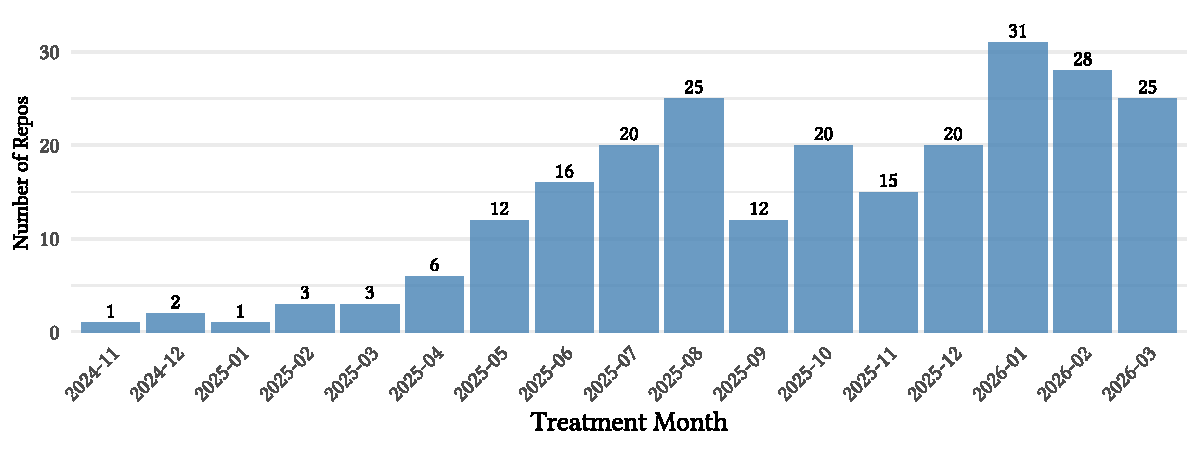
\includegraphics[width=\columnwidth]{../plots/treatment_timing.pdf}
\caption{Staggered adoption timing.
Each bar shows the number of repositories that first committed an AI configuration file in that month.
The 759 repositories that never adopted during the observation window serve as the control group for the difference-in-differences analysis.}
\label{fig:treatment-timing}
\end{figure}

\subsubsection{Before-and-After Comparison}
\label{sec:before-after}

The simplest within-unit estimator compares, for each treated repository, mean monthly commits (log-scale) before versus after the first AI configuration file commit.
This is the longitudinal analogue of the raw group comparison in Section~\ref{sec:naive-comparison}, but now within-unit rather than across units.
A paired $t$-test yields a mean change of $0.940$ (95\% CI $[0.710, 1.180]$), i.e., treated repositories see a 156\% ($\pm$31\%) increase in monthly commits after adoption.
The within-unit pairing absorbs all time-invariant confounders that plagued the cross-section---team skill, project type, organizational practices.
These factors are identical before and after adoption for the same repository, so they cannot drive the observed change.
However, this estimate is causal only if \emph{nothing else} about the treated repositories changed between the pre and post periods, besides the treatment itself.
In other words, the counterfactual outcome---what commits would have looked like without AI adoption---must have stayed flat.
This is a very strong assumption.
If all repositories are growing over 2024--2026 (e.g., due to platform growth, seasonal effects, or the general rise of AI-assisted development), then the before/after estimate captures the treatment effect \emph{plus} the secular trend.
The 156\% figure is almost certainly too high.
This motivates interrupted time series (ITS) analysis that models the trend explicitly.

\subsubsection{Interrupted Time Series (ITS)}
\label{sec:its}

ITS addresses the before/after comparison's key weakness by explicitly modeling the pre-treatment trend.
The regression specification is:
\begin{equation}
\label{eq:its}
Y_{it} = \alpha_i + \beta \cdot t + \delta \cdot \text{Post}_{it} + \gamma \cdot \text{TimeSince}_{it} + \varepsilon_{it}
\end{equation}
where $Y_{it}$ is $\log(1 + \text{monthly commits})$ for repository~$i$ in month~$t$; $\alpha_i$ is a repository fixed effect (one intercept per repository); $\beta \cdot t$ captures the common linear time trend; $\text{Post}_{it}$ equals~1 after adoption and~0 before; and $\text{TimeSince}_{it}$ counts months since adoption (zero before adoption), allowing the slope to change post-treatment.

Each term in Equation~\ref{eq:its} addresses a specific source of confounding.
The repository fixed effects $\alpha_i$ absorb \emph{all} time-invariant unobserved confounders---the exact variables (team skill, project culture, codebase complexity) that made the cross-sectional analysis in Section~\ref{sec:cross-sectional} non-credible.
The time trend $\beta \cdot t$ models a common linear secular trend, so the estimate of $\delta$ is purged of the trend that contaminated the before/after comparison.
ITS thus addresses \emph{two} of the cross-section's core problems simultaneously.
The coefficient $\delta$ tests for a discrete level shift at adoption, while $\gamma$ tests whether the post-treatment growth rate differs from the pre-treatment trend.

\begin{figure}[t]
  \centering
  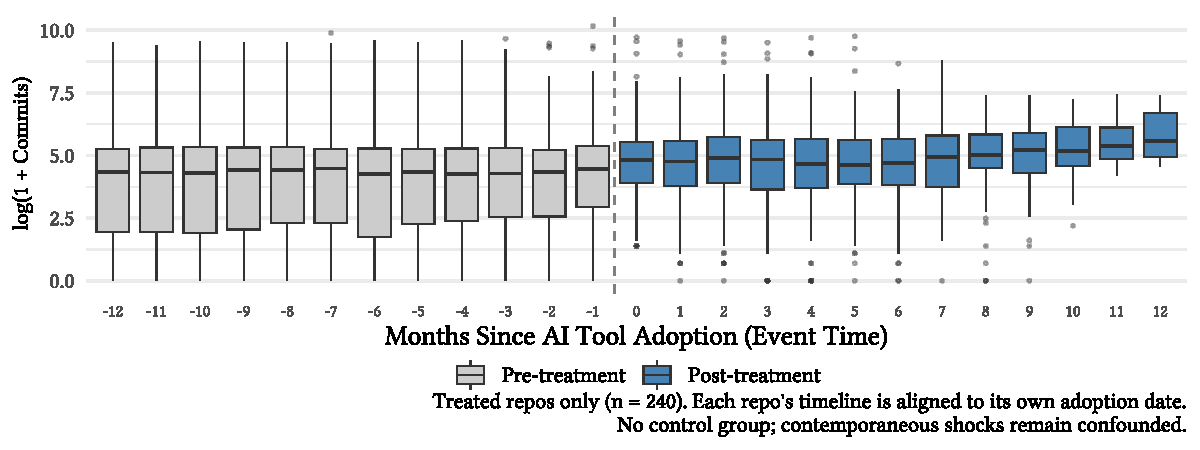
\includegraphics[width=\columnwidth]{../plots/its_boxplot.pdf}
  \caption{Distribution of $\log(1 + \text{monthly commits})$ by event time for treated repositories.
  Timelines are artificially aligned to each repository's own adoption date.
  ITS models the pre-treatment trend and tests for a level shift at adoption, but lacks a control group to distinguish the treatment effect from contemporaneous shocks.}
  \label{fig:its-boxplot}
\end{figure}

The level-shift estimate is $\hat{\delta} = 0.790$ (95\% CI $[0.550, 1.020]$), i.e., a 120\% ($\pm$26\%) increase.
This is lower than the before/after estimate (156\%), confirming that some of the before/after effect was driven by secular trends that ITS now absorbs.
For $\hat{\delta}$ to have a causal interpretation, the pre-treatment linear trend must be correctly specified, and no other event must systematically coincide with AI adoption.
Unlike the before/after comparison, ITS allows for a secular trend---but it assumes the trend is linear and that the \emph{only} thing that changes at the adoption date is the treatment itself.
Since ITS uses only treated repositories---there is no control group---any shock that happens around the adoption date is indistinguishable from the treatment effect: a team expansion, a major release, a GitHub platform change, or a field-wide shift in development practices.
If such events systematically co-occur with AI adoption, $\hat{\delta}$ absorbs them.
Additionally, if the true pre-treatment dynamics are nonlinear (e.g., accelerating growth from AI or decreasing effectiveness of AI), the linear trend specification may itself be misspecified.

One could address this limitation by adding a control group to the ITS specification---a design known as \emph{controlled interrupted time series} (CITS)~\cite{bernal2017interrupted}---but identification would still depend on correctly specifying the functional form of the trend for both groups.
Difference-in-differences offers a design-based alternative: Rather than modeling the trend explicitly, DiD \emph{differences out} common trends entirely in a natural experiment setting.
The parallel trends assumption (Section~\ref{sec:did}) requires only that treated and control units follow the \emph{same} trend---not that the trend take any particular functional form---making it less demanding than the parametric assumptions underlying ITS and CITS.

\subsubsection{Difference-in-Differences.}
\label{sec:did}

We now add an additional ``control'' group of 759 repositories that never adopted AI tools during the observation window.
An immediate objection arises: The na\"ive comparison in Section~\ref{sec:naive-comparison} showed that adopters and non-adopters differ dramatically in size, activity, and visibility.
How can such different repositories serve as a valid control group?
The answer lies in what DiD actually requires.
Because DiD compares \emph{changes} within each group, all time-invariant differences between groups---no matter how large---cancel out in the differencing.
A small hobbyist project and a large enterprise repository can serve as valid comparisons as long as their commit \emph{trends} would have evolved in parallel absent treatment.
DiD does not require the groups to look alike; it requires them to \emph{trend} alike (see a more formal discussion below).
The key idea is that any time-varying shock that affects both treated and control repositories equally is differenced out, \emph{even without modeling it explicitly}.

In the simplest case (one treatment group, one control group, two periods), the DiD estimator is:
\begin{equation}
\label{eq:did-2x2}
\hat{\tau}^{\text{DiD}} = \bigl(\bar{Y}^{\text{post}}_{\text{treated}} - \bar{Y}^{\text{pre}}_{\text{treated}}\bigr) - \bigl(\bar{Y}^{\text{post}}_{\text{control}} - \bar{Y}^{\text{pre}}_{\text{control}}\bigr)
\end{equation}
The first difference (within each pair of parentheses) removes unit fixed effects---just like the before/after comparison.
The second difference (between the two parentheses) removes common time shocks---exactly what ITS cannot do.
The double difference isolates the treatment effect (which is why it is called \emph{difference in differences}).

The two-way fixed effects (TWFE) regression specification expresses the same idea compactly:
\begin{equation}
\label{eq:twfe}
Y_{it} = \alpha_i + \gamma_t + \tau D_{it} + \varepsilon_{it}
\end{equation}
where $\alpha_i$ is an intercept (or fixed effect term) per repository and absorbs all time-invariant confounders (like ITS), $\gamma_t$ is a intercept per time period and absorbs \emph{common time shocks}, and $\hat{\tau}$ is the DiD estimate.
We present this specification for intuition only and do not report its estimate, for reasons we explain below.

The identifying assumption is \emph{parallel trends}:
\begin{equation}
\label{eq:parallel-trends}
E[Y_{it}(0) - Y_{is}(0) \mid \text{treated}] = E[Y_{it}(0) - Y_{is}(0) \mid \text{control}] \quad \forall\, t, s
\end{equation}
In plain language: absent treatment, treated and control repositories would have followed the same \emph{trend} in outcomes---so matching two groups on levels would be unnecessary if we can show that this assumption is plausible.
Parallel trends is weaker than the ITS assumption: Common shocks are fine as long as they affect both groups similarly.
It is also weaker than the before/after assumption: arbitrary trends are allowed, as long as they are parallel across groups.
We also require a \emph{no-anticipation assumption}: repositories do not change their behavior before they adopt AI tools.

In our setting, repositories adopt at different months, creating a \emph{staggered adoption} design.
Classic TWFE (Equation~\ref{eq:twfe}) implicitly uses already-treated repositories as controls for later-treated ones.
When treatment effects vary across cohorts or over time, this produces negative weights on some group-time ATTs, biasing $\hat{\tau}$~\cite{goodman2021difference, dechaisemartin2020two}.
This well-documented problem (see \citet{roth2023whats} for a survey) motivates modern estimators designed for staggered adoption with heterogeneous effects.
We apply two complementary modern DiD estimators that avoid the negative-weighting problem.

\textbf{Callaway \& Sant'Anna (2021) DiD}~\cite{callaway2021difference} is the most direct extension of the 2$\times$2 idea: it estimates separate treatment effects for each adoption cohort (group of repositories adopting in the same month), then aggregates.
For each cohort $g$ and time period $t$:
\begin{equation}
\label{eq:cs-att-gt}
ATT(g, t) = E[Y_t - Y_{g-1} \mid \text{cohort } g] - E[Y_t - Y_{g-1} \mid \text{never-treated}]
\end{equation}
This is a difference in outcome changes between cohort-$g$ repositories and never-treated repositories, measured from baseline~$g\!-\!1$.
We use no covariates, so this reduces to simple differences in means---the same double-differencing logic as Equation~\ref{eq:did-2x2}, applied separately to each cohort.
The overall ATT averages the group-time effects, weighting by cohort size.
The estimate is $\hat{\tau} = 0.416$ ($\text{SE} = 0.090$), i.e., 52\% ($\pm$14\%).
This unconditional specification relies on parallel trends holding \emph{without} conditioning on covariates.
The CS estimator also allows an alternative specification that conditions on pre-treatment covariates, which we do not report in this paper because of pre-trend violations.

\textbf{Borusyak et al.\ (2024) imputation DiD}~\cite{borusyak2024revisiting} estimates what outcomes \emph{would have been} without treatment, using a covariate-adjusted counterfactual model, then compares to what actually happened.
The procedure has three steps.
First, it fits a counterfactual model on all untreated observations (never-treated repositories plus pre-treatment periods of treated repositories):
\begin{equation}
\label{eq:borusyak-first-stage}
Y_{it} = \alpha_i + \gamma_t + X_{it}\beta + \varepsilon_{it} \quad \text{for all } (i,t) \text{ with } D_{it} = 0
\end{equation}
This includes time-varying covariates $X_{it}$: $\log$ of contributors, stars, issues, forks, and releases.
Second, for each treated observation, it plugs in the estimated coefficients to predict the counterfactual: $\hat{Y}_{it}(0) = \hat{\alpha}_i + \hat{\gamma}_t + X_{it}\hat{\beta}$.
Third, it computes the ATT as the average residual $\hat{\tau} = \text{mean}(Y_{it} - \hat{Y}_{it}(0))$ across all treated observations, weighting each treated (repository, month) cell equally.
Only untreated observations contribute to the counterfactual model; treated cells are never used as controls for other treated cells, avoiding the negative-weighting problem of TWFE\@.
The estimate is $\hat{\tau} = 0.281$ ($\text{SE} = 0.060$), i.e., 32\% ($\pm$8\%).\footnote{Doubly-robust and machine-learning-based DiD estimators~\cite{santanna2020doubly, chang2020double} further relax the linear functional-form assumption of Equation~\ref{eq:borusyak-first-stage}, but they share the same identifying assumption as Borusyak and would exhibit the same covariate-attenuation mechanism we describe below---the bottleneck is the role of the covariates in the DAG, not the flexibility of the estimator.}

\paragraph{Event Study and Pre-Trends Assessment.}
\label{sec:event-study}
Importantly, both estimators support event-study decompositions that estimate a separate treatment effect $\tau_k$ for each month~$k$ relative to adoption, which can be used to probe whether the parallel trend assumption is plausible (i.e., pre-trend tests).
Specifically, pre-treatment coefficients ($k < 0$) serve as a diagnostic and should be roughly around zero under parallel trends.
Post-treatment coefficients ($k \geq 0$) trace the dynamic treatment effect over time.

\begin{figure}[t]
  \centering
  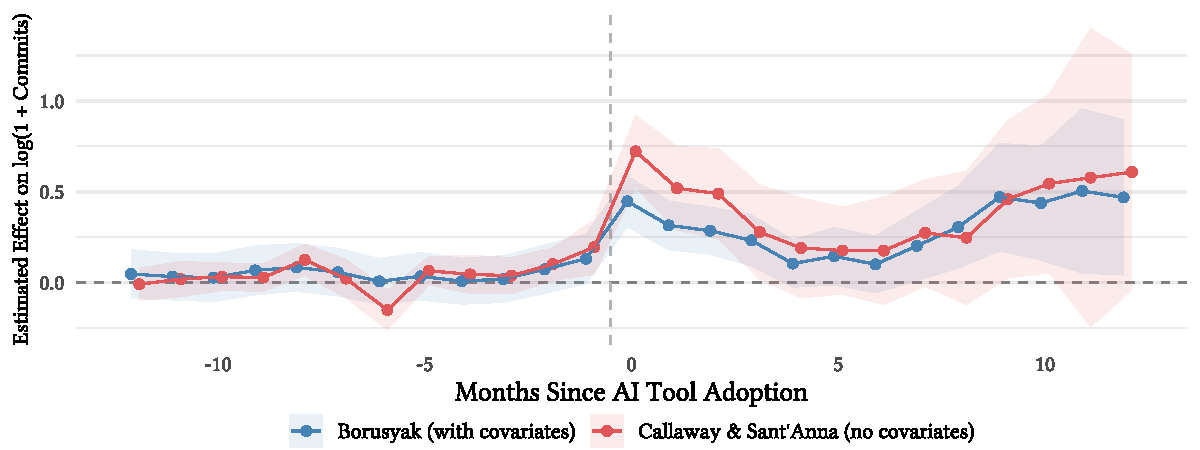
\includegraphics[width=\columnwidth]{../plots/event_study_comparison.pdf}
  \caption{Combined event study overlaying both DiD estimators.
  Pre-treatment coefficients near zero for both estimators support the parallel trends assumption.
  Post-treatment coefficients show the CS estimate (no covariates) consistently above the Borusyak estimate (with covariates), consistent with the covariate attenuation mechanism discussed in Section~\ref{sec:divergence}.
  Error bars show 95\% confidence intervals.}
  \label{fig:event-study}
  \end{figure}

Figure~\ref{fig:event-study} overlays the event-study estimates from both approaches.
Pre-treatment coefficients cluster near zero for both estimators, supporting the parallel trends assumption.
We assess pre-trends formally with two complementary tests.
For CS, we use simultaneous confidence bands from the \Code{did} package~\cite{callaway2021difference}, which control the family-wise error rate across all pre-treatment periods---a more conservative test than pointwise confidence intervals; 0 of 12 periods are significant under simultaneous bands.
For Borusyak, a joint Wald test pools the 12 pre-treatment coefficients ($H_0\!: \tau_{-12} = \cdots = \tau_{-1} = 0$; $p = 0.70$).\footnote{
It is important to note that passing a pre-trends test does not \emph{prove} parallel trends~\cite{roth2022pretest}.
A more principled alternative is the sensitivity analysis framework of \citet{rambachan2023more}, which asks: How large could post-treatment violations of parallel trends be, relative to any pre-trends we observe, before the conclusion reverses?
This shifts the burden from a binary pass/fail test to a continuous assessment of robustness.
}

\paragraph{Why Does the CS and Borusyak Estimator Diverge?}

The primary explanation is \textbf{covariate attenuation}---a direct application of the DAG reasoning from Section~\ref{sec:primer-dags}.
In the imputation step (Equation~\ref{eq:borusyak-first-stage}), the Borusyak model plugs in the \emph{post-treatment} values of the covariates $X_{it}$ to predict the counterfactual $\hat{Y}_{it}(0)$.
If AI adoption causes an increase in contributors or stars---because the tool makes the project more productive and visible---and those in turn drive more commits, then the covariates sit on the \emph{causal pathway}: adoption $\to$ covariates $\to$ commits.
Conditioning on them absorbs part of the treatment's effect, inflating the imputed counterfactual and shrinking the estimated ATT\@.
This is a concrete, numbers-in-hand instance of the mediator bias from Section~\ref{sec:primer-dags}: conditioning on a variable on the causal path between treatment and outcome attenuates the total effect (recall the discussion of colliders and mediators in the temporal DAG, Figure~\ref{fig:temporal-dag}).
The Borusyak estimate of 32\% captures only the effect of AI adoption that does \emph{not} flow through the covariates.
The CS specification omits covariates entirely, so it is unaffected by this mechanism.
Its estimate of 52\% targets the total effect under unconditional parallel trends---but this comes with its own trade-off: if parallel trends holds only \emph{conditional} on covariates, the unconditional estimate may be biased.

A secondary factor is \textbf{aggregation weights}: even without covariate attenuation, the two estimators would differ because they weight heterogeneous cohort-level effects differently---a well-known issue in the recent DiD literature~\cite{roth2023whats}.
Together, the pair of estimates brackets a plausible ATT range of 32--52\%, showing how methodological choices about covariate handling and aggregation can have substantive consequences.

\paragraph{Robustness.}
\label{sec:robustness}

We additionally probe two concerns about control group composition.
First, we trim structurally inactive repositories (fewer than 10 total commits) from the control group, since repositories with flat outcomes may violate parallel trends by failing to track the counterfactual trend of treated repositories.
The Borusyak ATT barely changes ($0.281 \to 0.280$), suggesting the result is not driven by inactive controls.
Second, we restrict the control group to repositories matched on pre-treatment observables via propensity score matching, yielding a similar estimate ($0.301$).
Both checks confirm that the DiD estimates are robust to control group composition.\footnote{Full details of the trimming and matching procedures are available in the replication notebook (Section~\ref{sec:data-availability}).}
These robustness checks probe specific threats to internal validity but cannot prove the identifying assumptions; they are best understood as ruling out specific alternative explanations (i.e., inactive controls or uncomparable control groups) as advocated in Section~\ref{sec:primer-stance}.

\paragraph{Longitudinal Takeaway.}
\label{sec:longitudinal-takeaway}

The longitudinal analysis demonstrates the power of design-based identification: by comparing the \emph{same} repository before and after AI adoption, every time-invariant confounder---team skill, project culture, codebase complexity---cancels out by construction, eliminating the single biggest threat to the cross-sectional analysis.
The three-stage progression from before/after (156\%) through ITS (120\%) to DiD (32--52\%) shows that each additional design element---trend modeling, a control group---shrinks the estimate substantially, indicating that secular trends and common shocks inflated the simpler estimates.
Within DiD, the CS--Borusyak comparison (52\% vs.\ 32\%) illustrates a subtle but important lesson: conditioning on post-treatment covariates that lie on the causal pathway attenuates the total effect---an instance of the mediator bias from Section~\ref{sec:primer-dags}.
The remaining threats---parallel trends violations, anticipation effects, and SUTVA violations---are \emph{more transparent and partially testable} (via event studies and pre-trends tests) than the ``all confounders measured'' assumption required by cross-sectional methods.
This transparency is the central advantage of design-based identification.

\paragraph{External Triangulation with Experimental Evidence.}
\label{sec:triangulation}

Beyond methodological defensibility, the DiD estimates gain credibility through comparison with independent experimental evidence on AI coding tools.
The closest construct-matched study is \citet{cui2025effects}, which pools three firm-level field randomized trials ($N = 4{,}867$ developers at Microsoft, Accenture, and a Fortune-100 company) and reports a $+26\%$ increase in completed tasks ($\text{SE} \approx 10\%$).
Shorter-horizon controlled task experiments find larger per-task speedups---\citet{peng2023impact} report a $55.8\%$ reduction in task-completion time on a single JavaScript task ($N = 95$), and \citet{DBLP:conf/icse-seip/ParadisGMNMMZFC25} report an $\approx 21\%$ time reduction on an enterprise coding task at Google ($N = 96$)---though these measure task speed rather than sustained output volume, so their magnitudes are not directly comparable to monthly commits.
The experimental evidence is not uniformly positive: \citet{becker2025measuring} report a $+19\%$ \emph{slowdown} on 16 experienced maintainers working on 246 issues in mature open-source repositories, and a follow-up with late-2025 data reversed the direction (non-significant speedups of $-4\%$ to $-18\%$) but was flagged by its authors as unreliable due to control-arm attrition~\cite{metr2026uplift}, leaving the effect on experienced open-source maintainers of mature codebases poorly identified as of early 2026.
Our $+32\%$ to $+52\%$ ATT is consistent with the firm-level RCT anchor of \citet{cui2025effects} and sits within the broader range established by these controlled experiments; the na\"ive cross-sectional $+911\%$ is inconsistent with every RCT on record by roughly an order of magnitude.
External triangulation does not validate our DiD estimate in a construct-matched sense---task-time and commit-volume outcomes differ, and open-source and enterprise populations differ---but it shows that the design-based and controlled-experimental evidence agree on the plausible magnitude range, while the na\"ive cross-sectional estimate does not.

\subsection{Summary}
\label{sec:summary}

\begin{table*}[t]
\centering
\caption{Summary of all effect estimates from the cross-sectional (Section~\ref{sec:cross-sectional}) and longitudinal (Section~\ref{sec:longitudinal}) analyses.
The estimate is on the $\log(1 + \text{monthly commits})$ scale; the percentage change is $(e^{\text{Estimate}} - 1) \times 100\%$, with $\pm$ computed via the delta method ($e^{\text{Estimate}} \times \text{SE} \times 100\%$).
All OLS specifications approximate the ATE; PSM, IPW, and all longitudinal methods target the ATT.}
\label{tab:all-estimates}
\small
\begin{tabular}{llrrr}
\toprule
Method & Identifying assumption & Estimate & SE & \% change \\
\midrule
\multicolumn{5}{l}{\emph{Cross-sectional (Section~\ref{sec:cross-sectional})}} \\
Na\"ive comparison (no controls) & As-if random assignment & 2.314 & 0.124 & +911\% ($\pm$125\%) \\
Kitchen-sink OLS (snapshot covariates) & Cond.\ ignorability (temporally ambiguous) & 0.946 & 0.116 & +158\% ($\pm$30\%) \\
OLS (DAG-justified, pre-treatment) & Cond.\ ignorability (pre-treatment) & 0.696 & 0.090 & +101\% ($\pm$18\%) \\
PSM (1:1 NN) & Cond.\ ignorability (pre-treatment) & 0.574 & 0.094 & +78\% ($\pm$17\%) \\
IPW (ATT) & Cond.\ ignorability (pre-treatment) & 0.509 & 0.091 & +66\% ($\pm$15\%) \\
\addlinespace
\multicolumn{5}{l}{\emph{Longitudinal (Section~\ref{sec:longitudinal})}} \\
Before/after & Counterfactual outcome stays flat & 0.940 & 0.120 & +156\% ($\pm$31\%) \\
ITS with repo FE & Correct trend; no contemporaneous shocks & 0.790 & 0.120 & +120\% ($\pm$26\%) \\
DiD: CS (no covariates) & Parallel trends (unconditional) & 0.416 & 0.090 & +52\% ($\pm$14\%) \\
DiD: Borusyak (with covariates) & Parallel trends (conditional on $X_{it}$) & 0.281 & 0.060 & +32\% ($\pm$8\%) \\
\bottomrule
\end{tabular}
\end{table*}

Table~\ref{tab:all-estimates} compares all estimates from Sections~\ref{sec:cross-sectional} and~\ref{sec:longitudinal}, along with each method's identifying assumption and its key vulnerability.
It is important to note that the \emph{design} matters more than the estimator.
The na\"ive comparison ($+911\%$) drops to $+158\%$ once we add snapshot controls, and further to $+101\%$ once we condition only on pre-treatment confounders justified by the temporal DAG---each step removes a different source of bias.
Yet within the DAG-justified cross-section, switching from OLS to PSM to IPW still yields esimates higher than the DiD estimates: All three share the conditional ignorability assumption which is violated by the unobserved confounders that no GitHub API data can capture.
Across longitudinal designs, the estimates change dramatically: the before/after estimate (156\%) drops to 120\% with ITS (which absorbs secular trends) and further to 32--52\% with DiD (which absorbs common shocks via a control group).
Each step trades a strong assumption for a weaker one, and the estimates shrink accordingly.
The identifying assumption is progressively weaker and more plausible as we move from the cross-sectional to the longitudinal designs.
The design-based estimates are not only methodologically defensible; they are also the only estimates in Table~\ref{tab:all-estimates} consistent with the magnitude range reported by field experiments on AI coding tools (Section~\ref{sec:triangulation}).
